\documentclass[11pt,a4paper]{article}

% Packages
\usepackage[utf8]{inputenc}
\usepackage[T1]{fontenc}
\usepackage{amsmath,amssymb}
\usepackage{graphicx}
\usepackage{booktabs}
\usepackage{hyperref}
\usepackage[margin=1in]{geometry}
\usepackage{caption}
\usepackage{subcaption}
\usepackage{listings}
\usepackage{xcolor}
\usepackage{float}

% Code listing style
\lstset{
    basicstyle=\ttfamily\small,
    breaklines=true,
    frame=single,
    backgroundcolor=\color{gray!10},
    keywordstyle=\color{blue},
    commentstyle=\color{green!50!black},
}

\title{SL-GPS Validation Report:\\Methyl Formate (CH$_3$OCHO) Mechanism Reduction\\via Supervised Learning --- ThInK 1.0}
\author{SL-GPS Automated Validation Framework}
\date{\today}

\begin{document}

\maketitle

\begin{abstract}
This report presents a validation of the Supervised Learning -- Global Pathway Selection (SL-GPS) method for adaptive chemical mechanism reduction applied to methyl formate (CH$_3$OCHO) combustion using the ThInK~1.0 mechanism (160 species, 1089 reactions). The complete pipeline is documented: training data generation via GPS, neural network training, and validation against the detailed mechanism across 8 test cases spanning temperatures of 800--1500~K, pressures of 1--20~atm, and equivalence ratios of 0.7--1.3. All training parameters, species classifications, and results are reported for full reproducibility.
\end{abstract}

\tableofcontents
\newpage

% =============================================================================
\section{Introduction}
% =============================================================================

The SL-GPS method trains neural networks on Global Pathway Selection (GPS) data to dynamically predict which chemical species are important during combustion simulations. At each timestep, the ANN evaluates the current thermochemical state and activates only the predicted species, producing an adaptive reduced mechanism that varies in size throughout the simulation.

This report validates SL-GPS on the ThInK~1.0 mechanism \cite{think1} for methyl formate (CH$_3$OCHO, also known as methyl methanoate), a simple oxygenated fuel of interest as a biodiesel surrogate and a key intermediate in dimethyl ether (DME) and dimethoxymethane (DMM) oxidation.

\subsection{Mechanism Overview}

\begin{table}[H]
\centering
\caption{ThInK 1.0 mechanism summary.}
\label{tab:mech}
\begin{tabular}{ll}
\toprule
\textbf{Property} & \textbf{Value} \\
\midrule
Name & ThInK 1.0 \\
Species & 160 \\
Reactions & 1089 \\
Target fuels & C$_1$--C$_3$ oxygenated fuels \\
Format & Cantera YAML \\
\bottomrule
\end{tabular}
\end{table}

% =============================================================================
\section{Methodology}
\label{sec:methodology}
% =============================================================================

\subsection{SL-GPS Pipeline}

The pipeline consists of three stages:
\begin{enumerate}
    \item \textbf{Data generation:} Run $N$ autoignition simulations with randomized initial conditions ($T$, $P$, $\phi$). At each timestep interval, apply GPS ($\alpha = 0.001$) to label which species are important.
    \item \textbf{ANN training:} Train an ensemble of neural networks on the GPS-labeled data. Select the best model by validation loss.
    \item \textbf{Validation:} Run new autoignition cases with the detailed mechanism and simultaneously with SL-GPS (ANN-guided reduction). Compare temperature, HRR, species profiles, and ignition delay.
\end{enumerate}

\subsection{Species Classification}

Before training, species are partitioned into three groups based on occurrence frequency in the GPS training data:
\begin{itemize}
    \item \textbf{Always} ($>99\%$ occurrence): unconditionally included in all reduced mechanisms
    \item \textbf{Variable} (1--99\%): predicted by the ANN at each timestep
    \item \textbf{Never} ($<1\%$ occurrence): permanently excluded
\end{itemize}
Only the \emph{variable} species are outputs of the neural network.

\subsection{Neural Network Architecture}

\begin{itemize}
    \item \textbf{Input:} temperature, pressure, and 14 selected species mole fractions (normalized via MinMaxScaler)
    \item \textbf{Hidden layers:} 2 fully-connected layers $\times$ 32 neurons with ReLU activation
    \item \textbf{Output:} sigmoid activation (one output per variable species)
    \item \textbf{Loss:} binary cross-entropy; \textbf{Optimizer:} Adam
    \item \textbf{Training:} ensemble of 8 models in parallel, best selected by validation loss
    \item \textbf{Early stopping:} patience = 30 epochs, max = 200 epochs
\end{itemize}

% =============================================================================
\newpage
\section{CH\texorpdfstring{$_3$}{3}OCHO --- ThInK 1.0}
\label{sec:ch3ocho}
% =============================================================================

\subsection{Training Configuration}

\begin{table}[H]
\centering
\caption{CH$_3$OCHO training configuration summary.}
\label{tab:ch3ocho_config}
\begin{tabular}{ll}
\toprule
\textbf{Parameter} & \textbf{Value} \\
\midrule
\multicolumn{2}{l}{\textit{Mechanism}} \\
\quad Mechanism & ThInK 1.0 \\
\quad Species / Reactions & 160 / 1089 \\
\midrule
\multicolumn{2}{l}{\textit{Data Generation}} \\
\quad Training cases & 15 (parallel execution) \\
\quad Temperature range & 800--1600~K (uniform) \\
\quad Pressure range & 1--20~atm (log-uniform) \\
\quad Equivalence ratio $\phi$ & 0.7--1.4 (uniform) \\
\quad GPS $\alpha$ & 0.001 \\
\quad Total training samples & 707 \\
\midrule
\multicolumn{2}{l}{\textit{Species Classification}} \\
\quad Always species & 14 (unconditionally included) \\
\quad Variable species (ANN outputs) & 63 \\
\quad Never species & 83 (permanently excluded) \\
\midrule
\multicolumn{2}{l}{\textit{ANN Training}} \\
\quad Input features & $T$, $P$ + 14 species mole fractions \\
\quad Architecture & 2 hidden layers $\times$ 32 neurons \\
\quad Ensemble size & 8 parallel trainings \\
\quad Max epochs / Early stopping & 200 / patience 30 \\
\bottomrule
\end{tabular}
\end{table}

\textbf{Input species (ANN features):} CH$_3$OCHO, O$_2$, H$_2$O, CO$_2$, CO, OH, H, H$_2$, CH$_4$, CH$_2$O, CH$_3$OH, HO$_2$, CH$_3$O, HCO

\subsection{Validation Cases}

\begin{table}[H]
\centering
\caption{CH$_3$OCHO validation conditions (4 baseline + 4 extended).}
\label{tab:ch3ocho_cases}
\begin{tabular}{lcccc}
\toprule
\textbf{Case} & \textbf{$T_0$ (K)} & \textbf{$P$ (atm)} & \textbf{$\phi$} & \textbf{$t_{\text{end}}$ (s)} \\
\midrule
T1000\_P1 & 1000 & 1 & 1.0 & 0.1 \\
T1200\_P1 & 1200 & 1 & 1.0 & 0.01 \\
T1200\_P10 & 1200 & 10 & 1.0 & 0.005 \\
T1500\_P1 & 1500 & 1 & 1.0 & 0.002 \\
\midrule
\multicolumn{5}{c}{\textit{Extended cases (difficult conditions)}} \\
\midrule
T800\_P20 & 800 & 20 & 1.0 & 0.5 \\
T900\_P10 & 900 & 10 & 1.0 & 0.5 \\
T1100\_P1\_rich & 1100 & 1 & 1.3 & 0.05 \\
T1400\_P5\_lean & 1400 & 5 & 0.7 & 0.01 \\
\bottomrule
\end{tabular}
\end{table}

\subsection{Results --- Baseline Cases}

\begin{figure}[H]
    \centering
    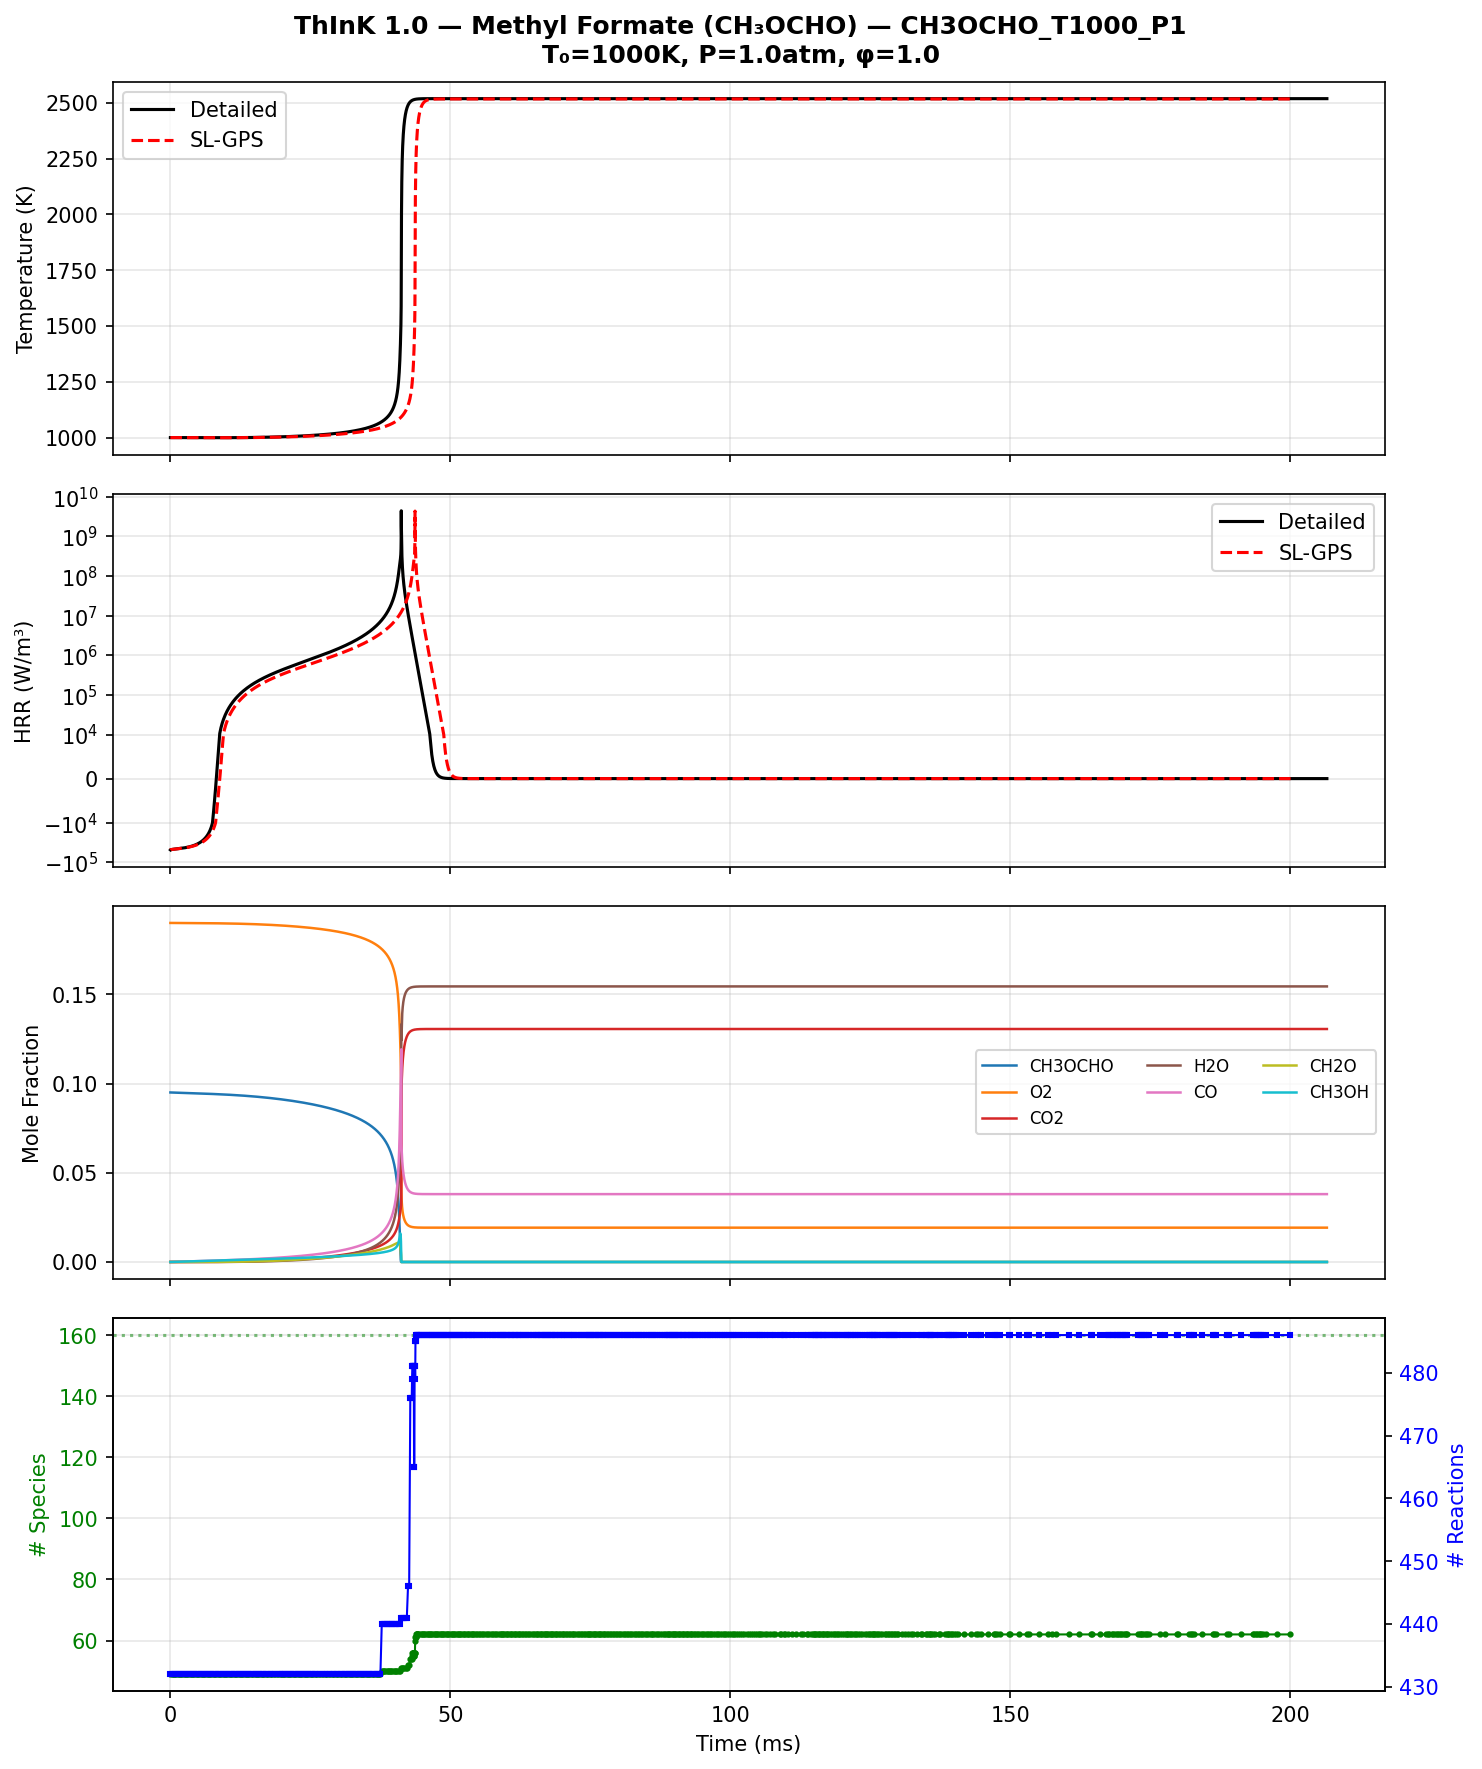
\includegraphics[width=0.95\textwidth]{results/ch3ocho/CH3OCHO_T1000_P1.png}
    \caption{CH$_3$OCHO Case 1: $T_0=1000$~K, $P=1$~atm, $\phi=1.0$. Ignition delay error: 6.0\%.}
    \label{fig:ch3ocho_case1}
\end{figure}

\begin{figure}[H]
    \centering
    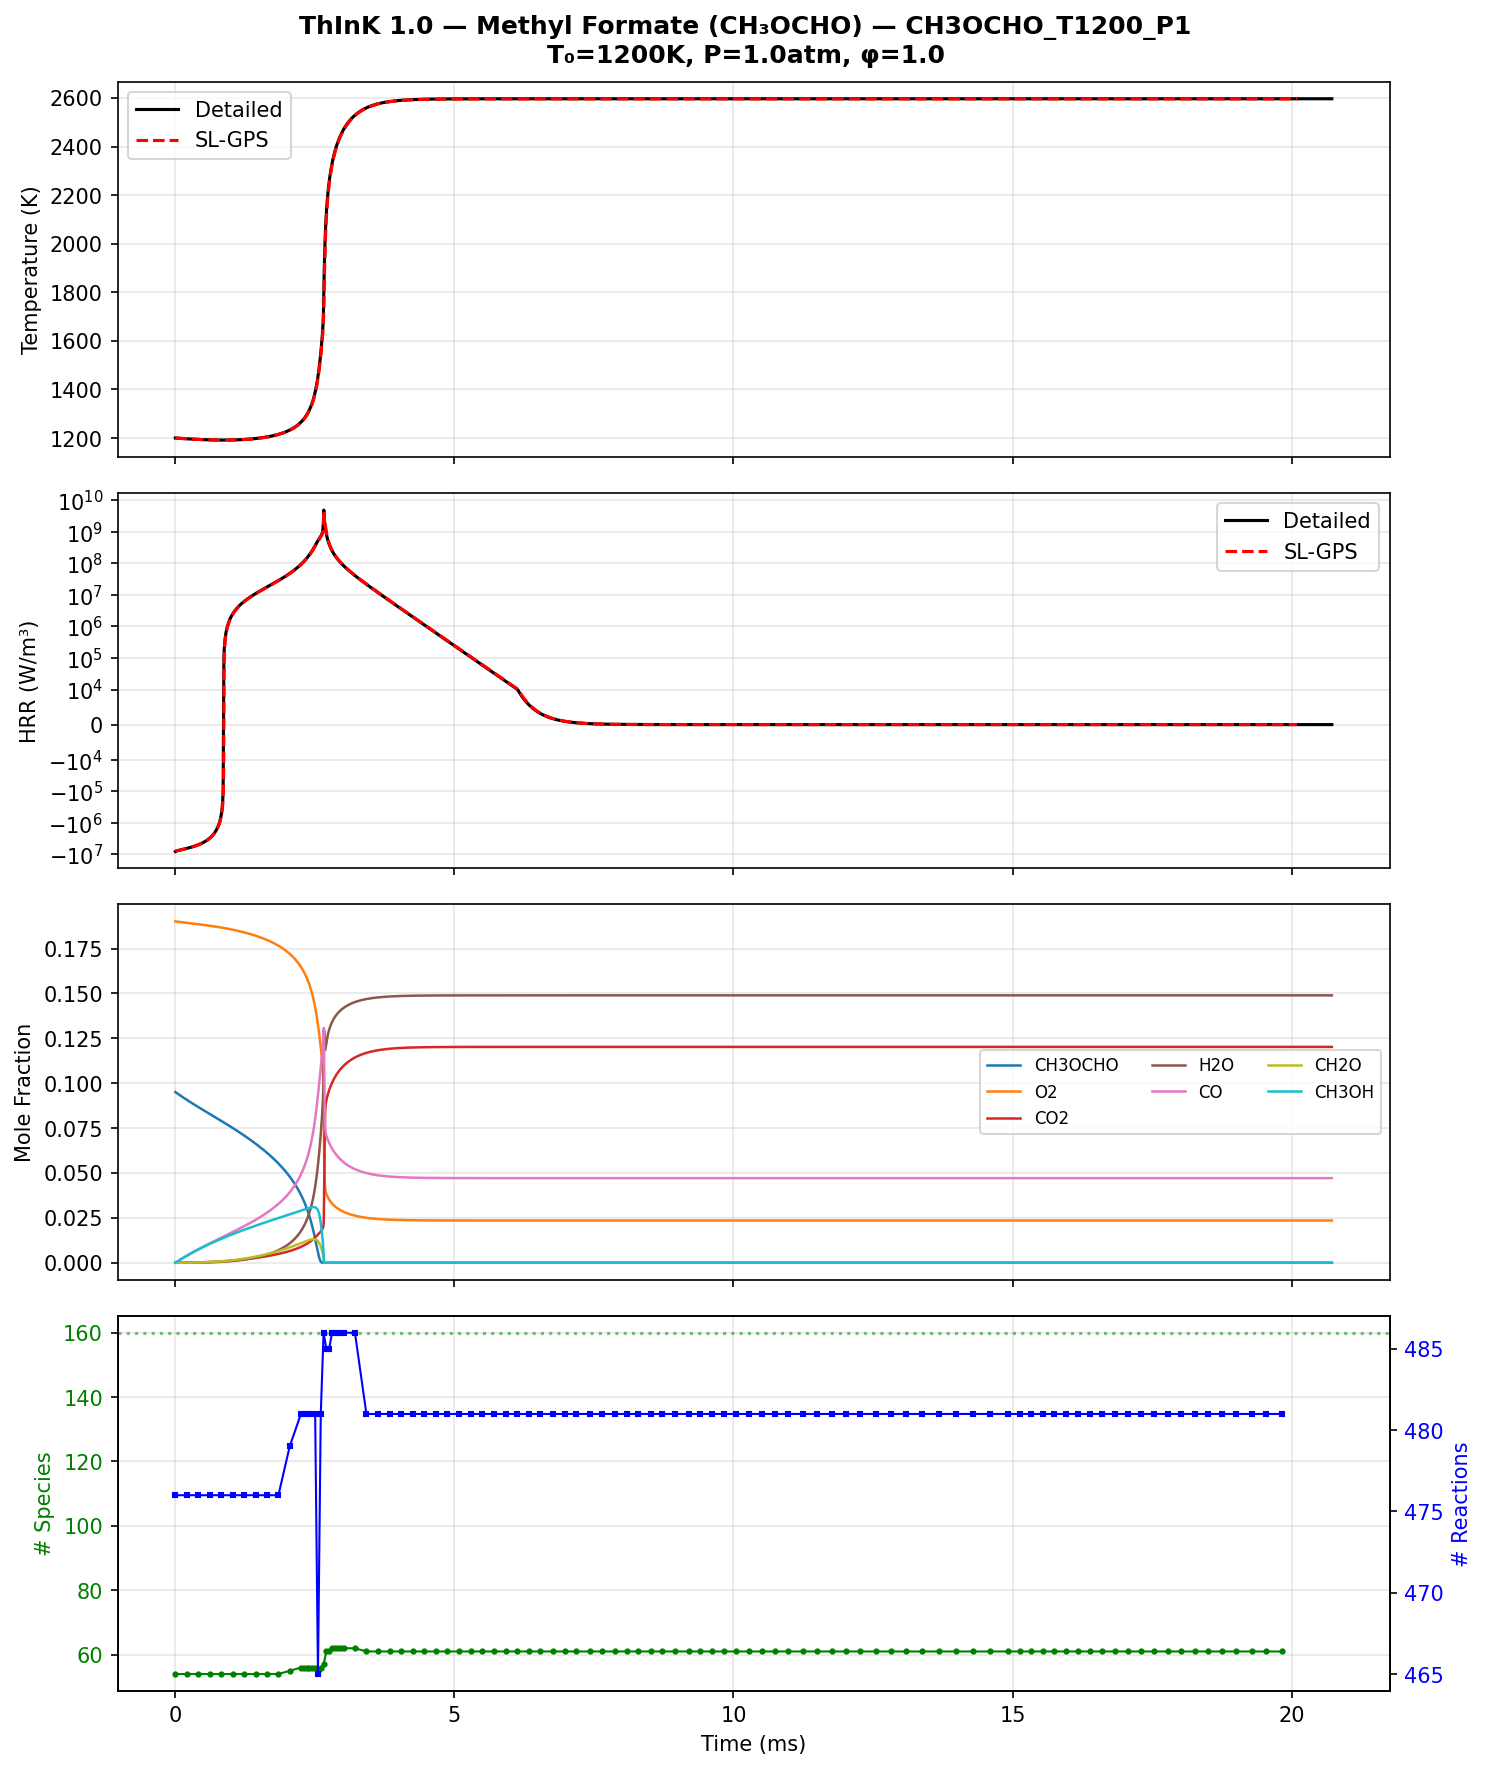
\includegraphics[width=0.95\textwidth]{results/ch3ocho/CH3OCHO_T1200_P1.png}
    \caption{CH$_3$OCHO Case 2: $T_0=1200$~K, $P=1$~atm, $\phi=1.0$. Ignition delay error: 0.2\%.}
    \label{fig:ch3ocho_case2}
\end{figure}

\begin{figure}[H]
    \centering
    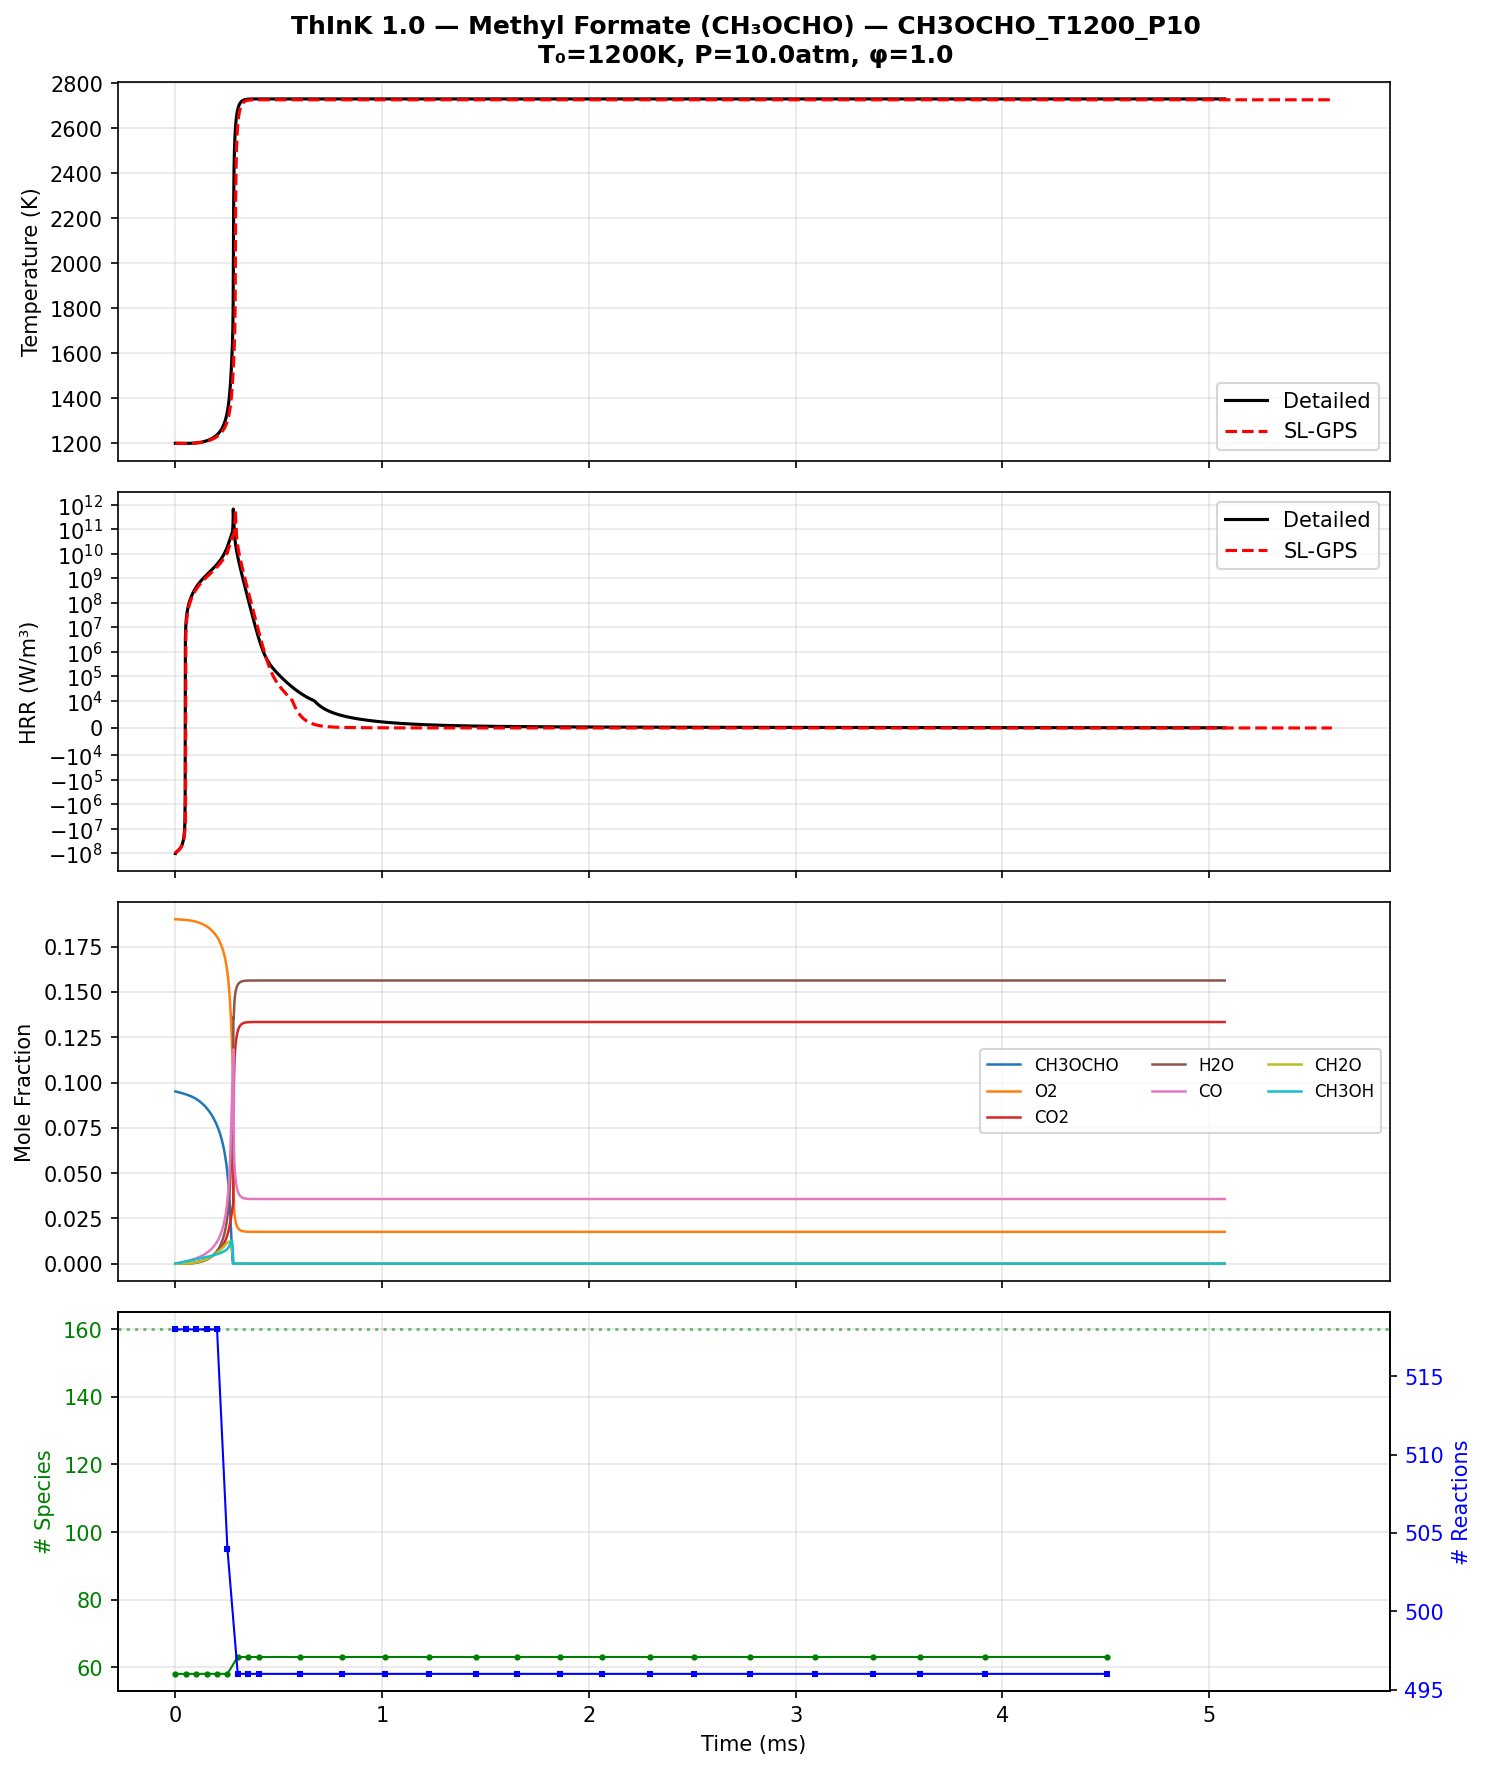
\includegraphics[width=0.95\textwidth]{results/ch3ocho/CH3OCHO_T1200_P10.png}
    \caption{CH$_3$OCHO Case 3: $T_0=1200$~K, $P=10$~atm, $\phi=1.0$. Ignition delay error: 3.4\%.}
    \label{fig:ch3ocho_case3}
\end{figure}

\begin{figure}[H]
    \centering
    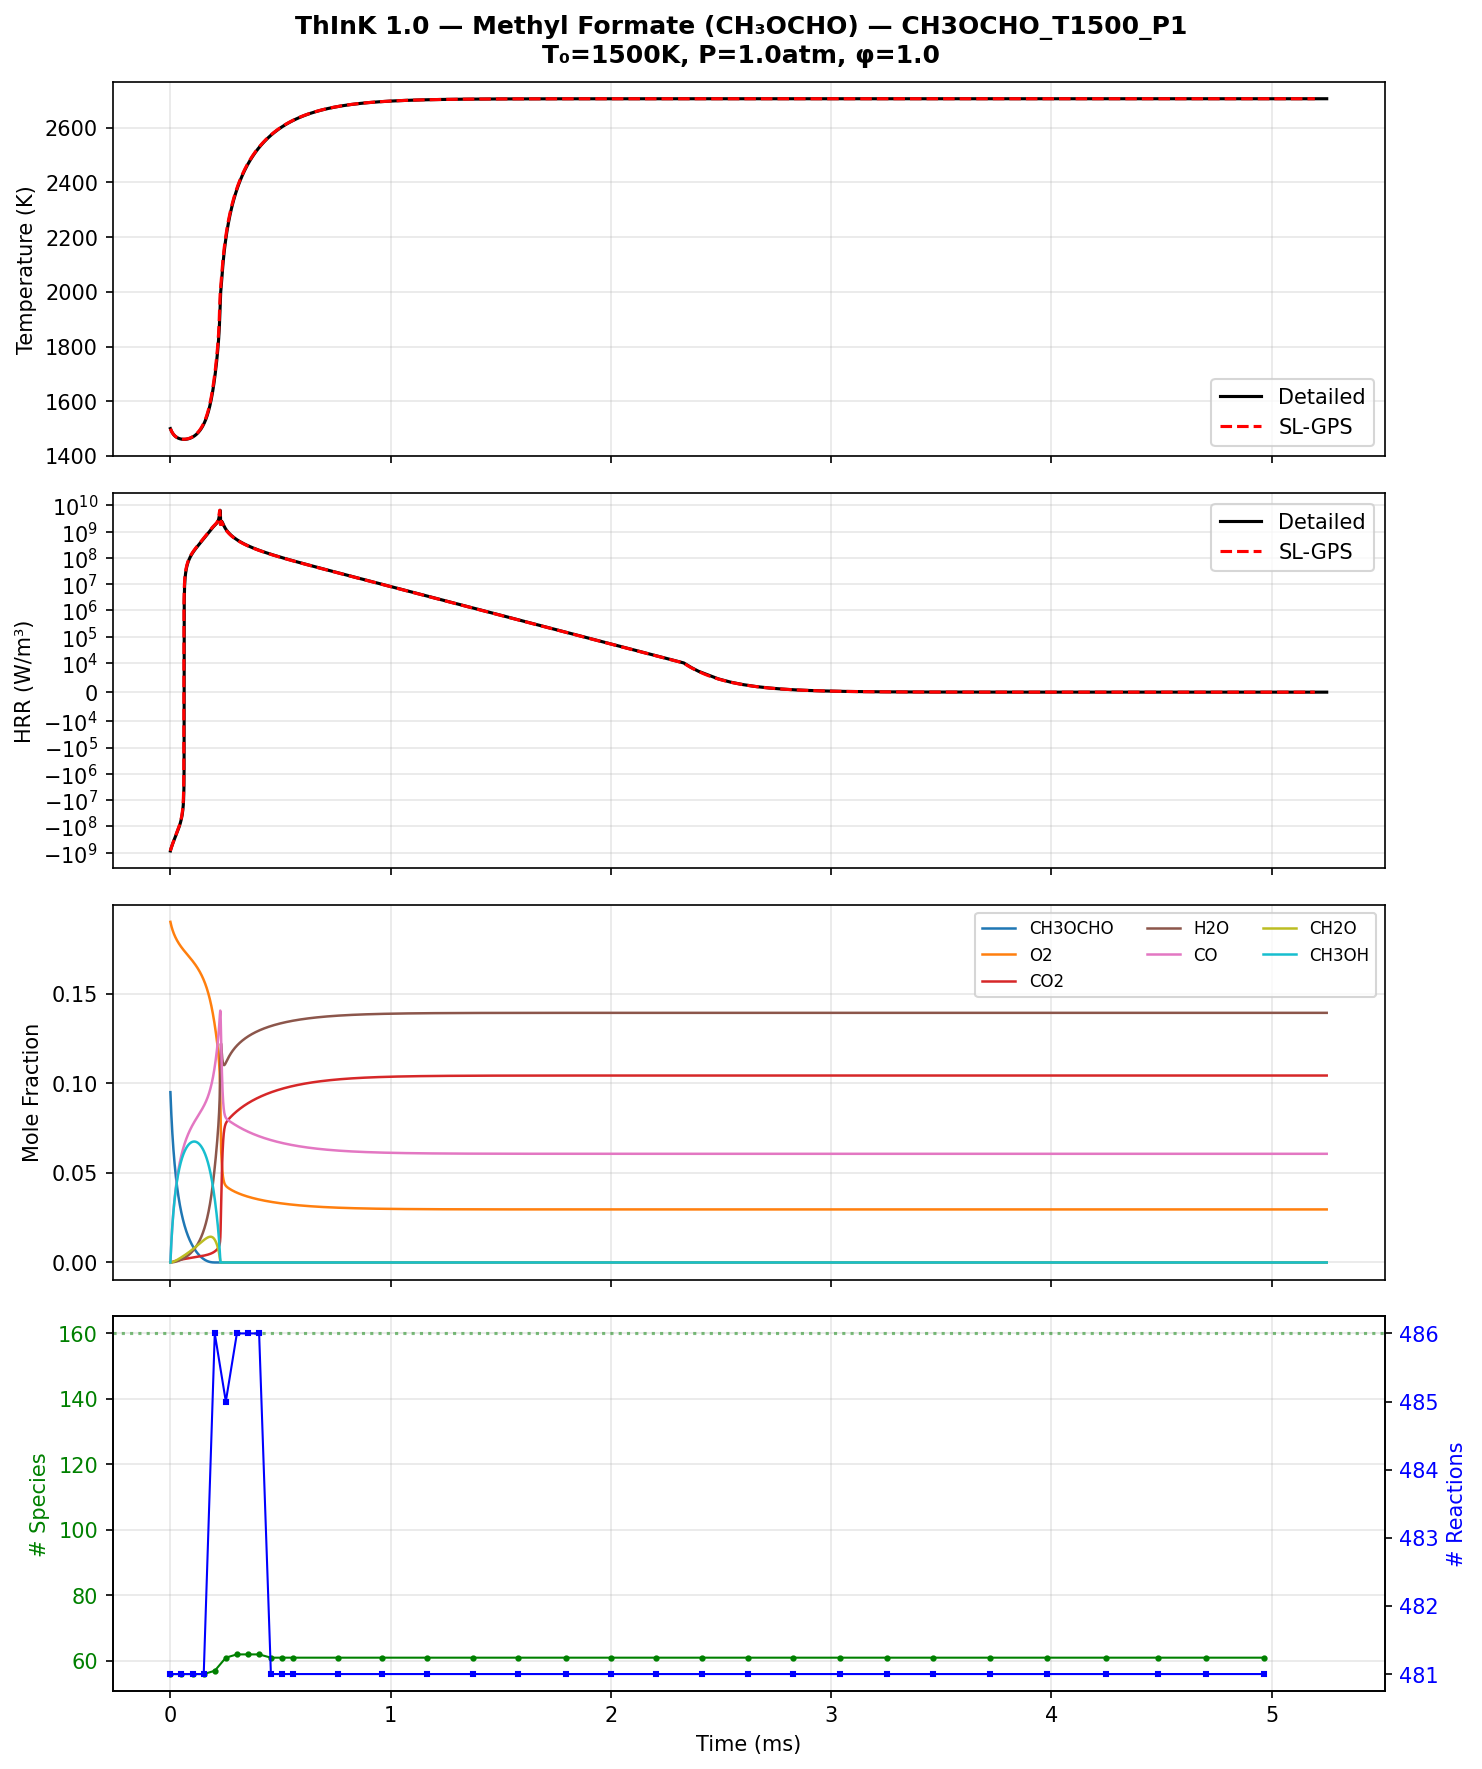
\includegraphics[width=0.95\textwidth]{results/ch3ocho/CH3OCHO_T1500_P1.png}
    \caption{CH$_3$OCHO Case 4: $T_0=1500$~K, $P=1$~atm, $\phi=1.0$. Ignition delay error: 0.9\%.}
    \label{fig:ch3ocho_case4}
\end{figure}

\subsection{Results --- Extended Cases}

\begin{figure}[H]
    \centering
    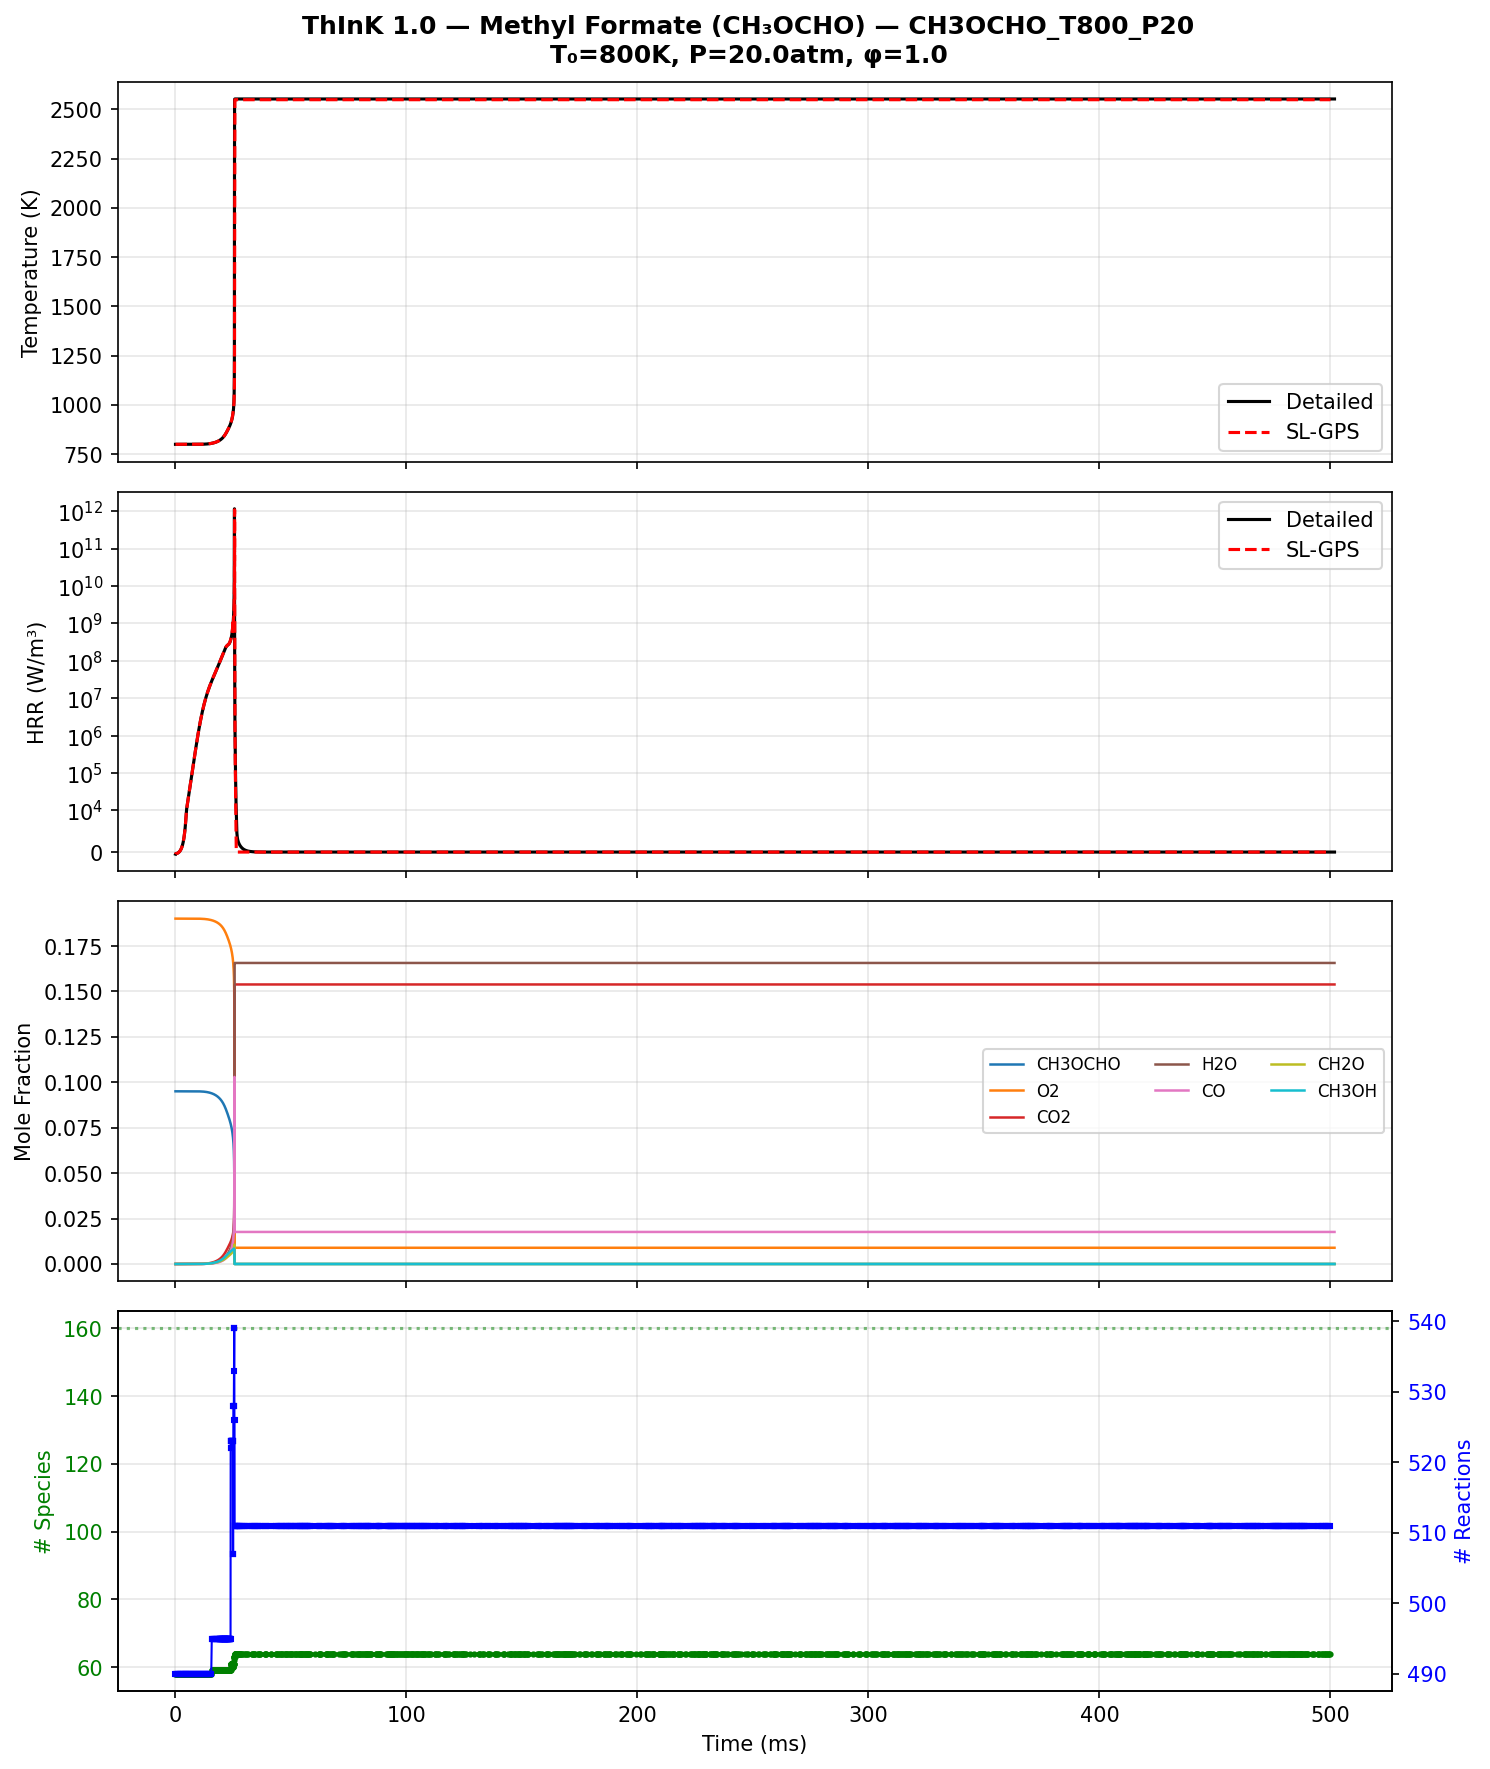
\includegraphics[width=0.95\textwidth]{results/ch3ocho/CH3OCHO_T800_P20.png}
    \caption{CH$_3$OCHO Case 5: $T_0=800$~K, $P=20$~atm, $\phi=1.0$. Ignition delay error: 0.3\%.}
    \label{fig:ch3ocho_case5}
\end{figure}

\begin{figure}[H]
    \centering
    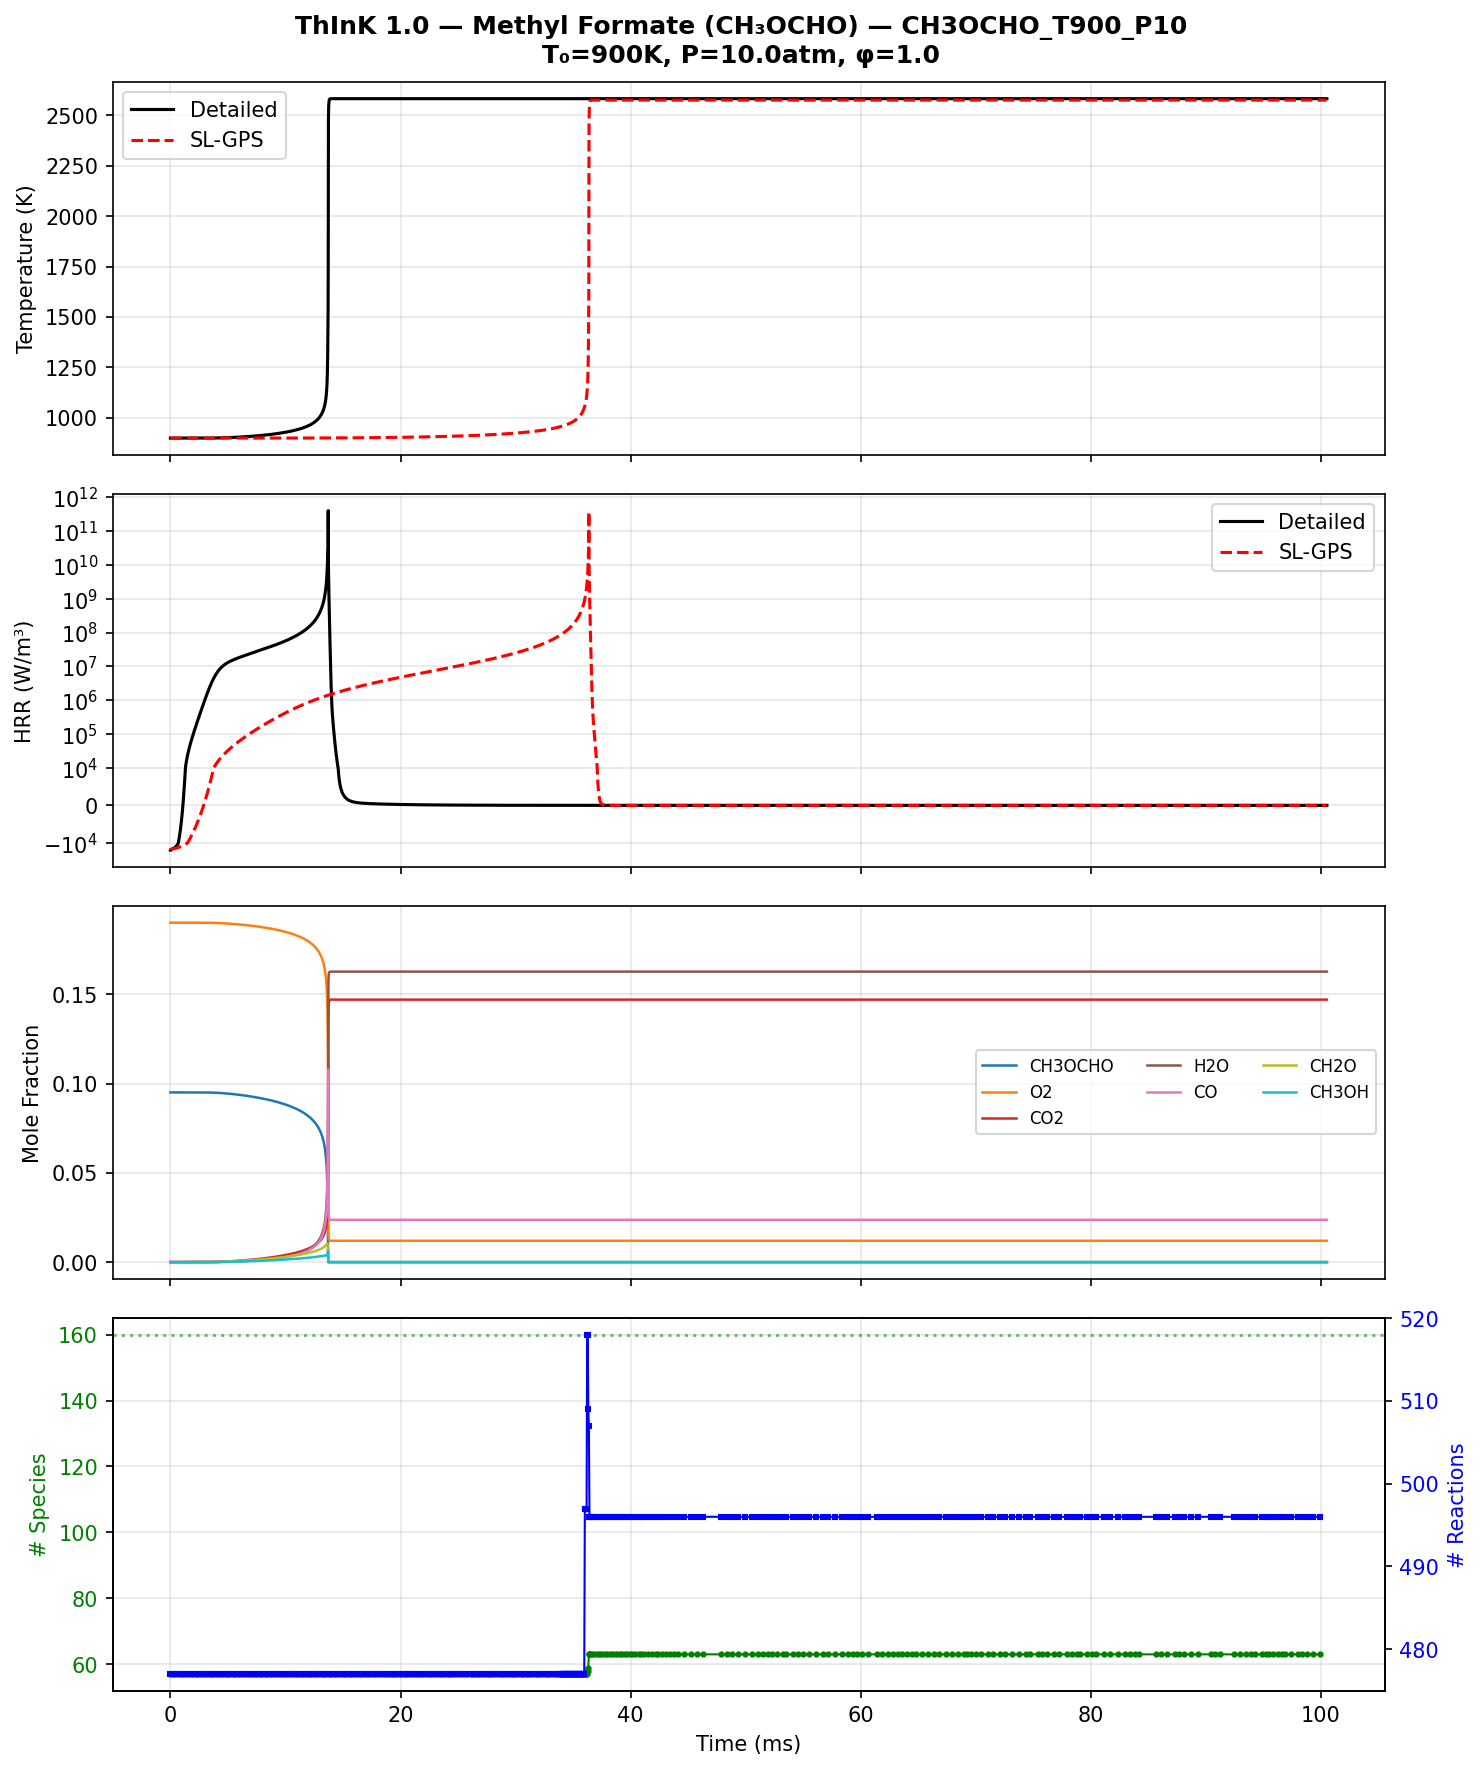
\includegraphics[width=0.95\textwidth]{results/ch3ocho/CH3OCHO_T900_P10.png}
    \caption{CH$_3$OCHO Case 6: $T_0=900$~K, $P=10$~atm, $\phi=1.0$. Ignition delay error: 165.2\%. \textbf{Failed} --- low-temperature NTC regime insufficiently covered by training data.}
    \label{fig:ch3ocho_case6}
\end{figure}

\begin{figure}[H]
    \centering
    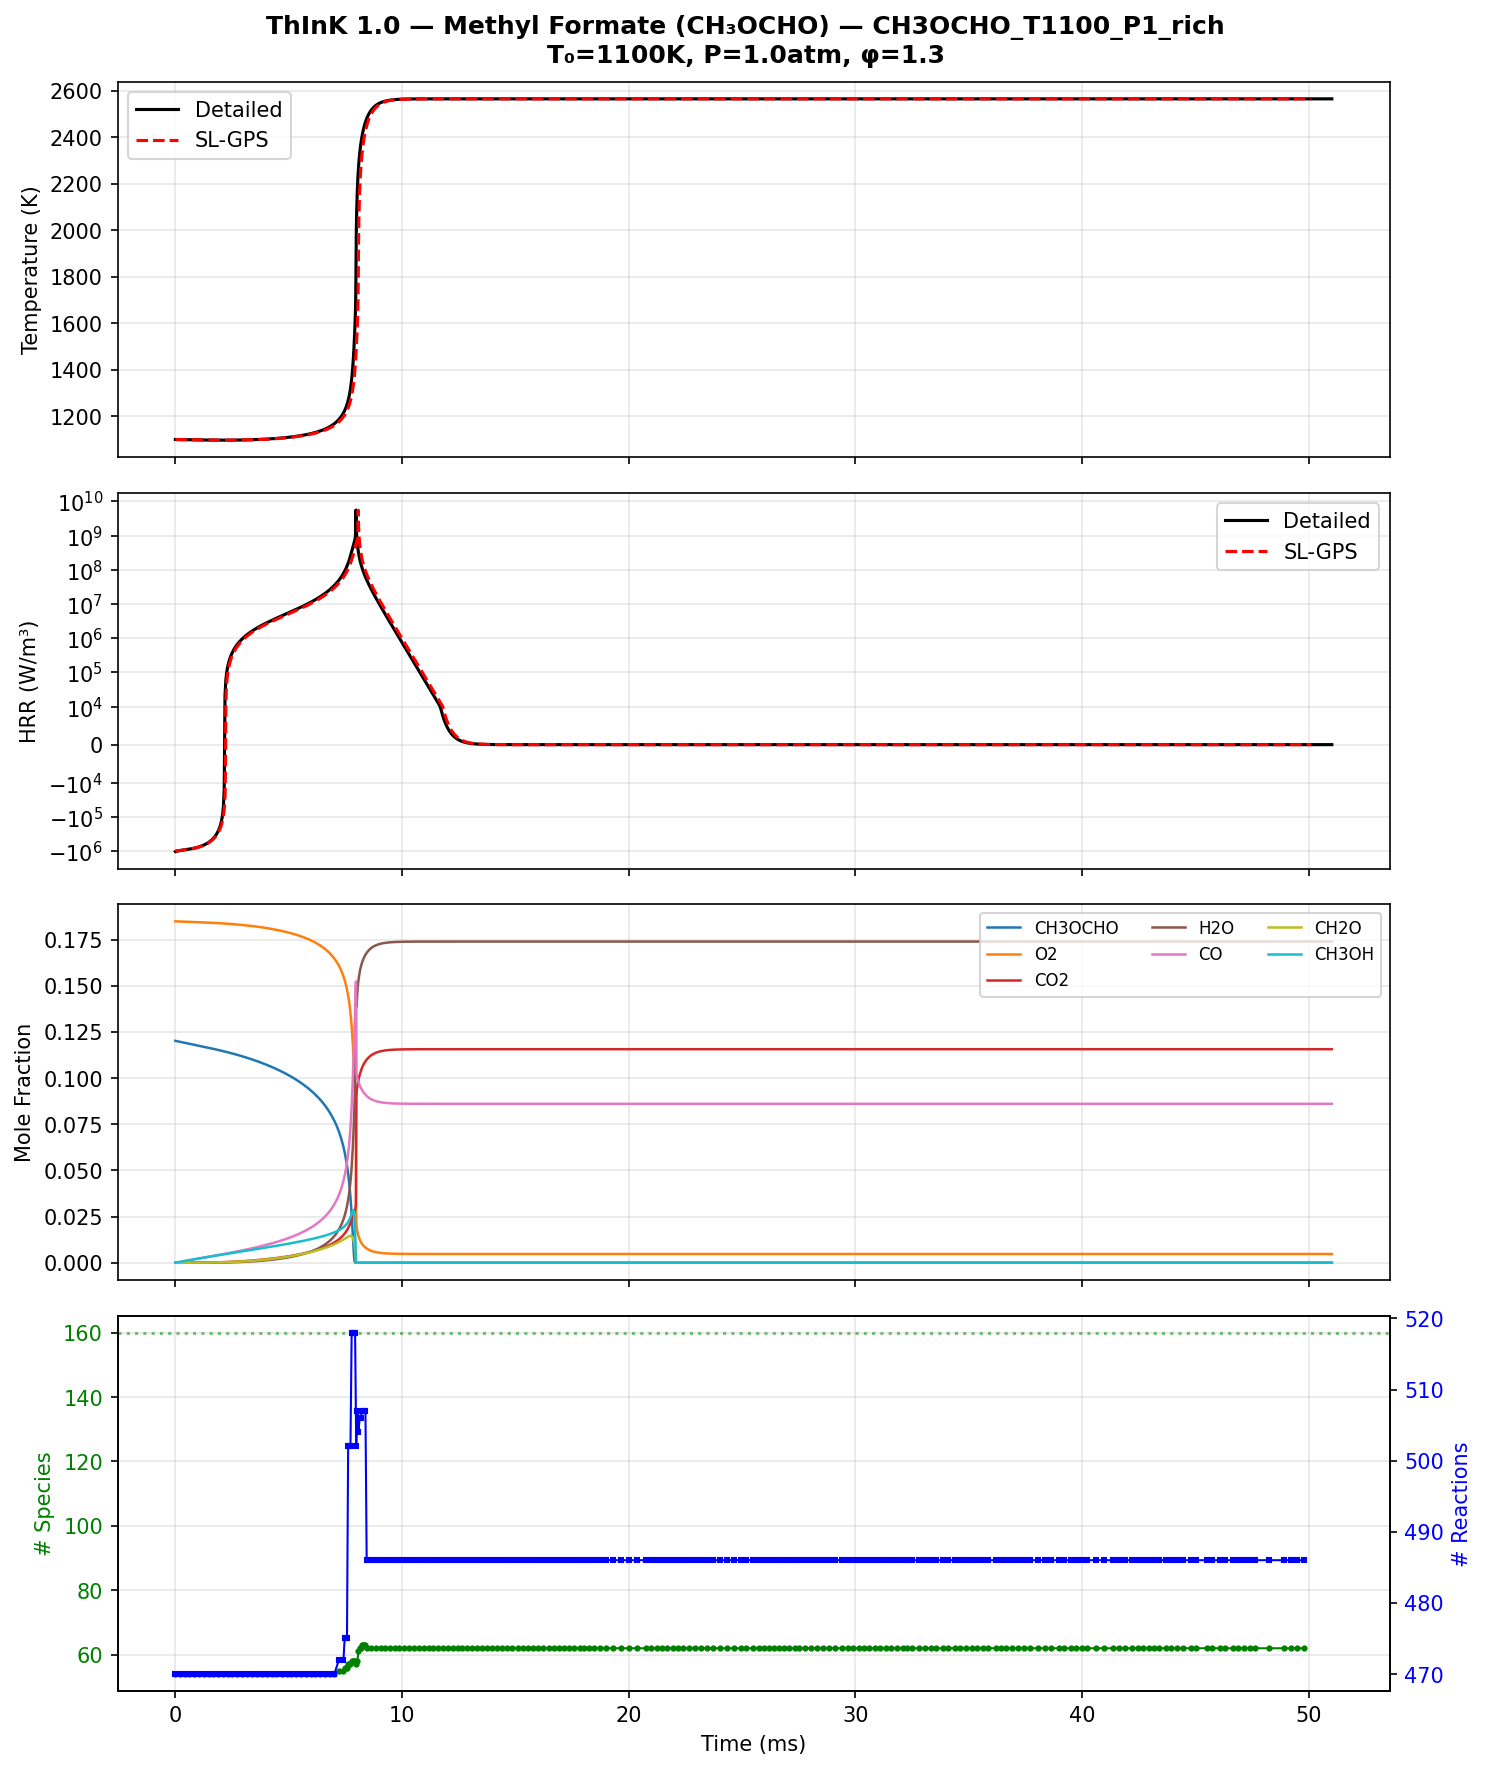
\includegraphics[width=0.95\textwidth]{results/ch3ocho/CH3OCHO_T1100_P1_rich.png}
    \caption{CH$_3$OCHO Case 7: $T_0=1100$~K, $P=1$~atm, $\phi=1.3$. Fuel-rich. Ignition delay error: 1.3\%.}
    \label{fig:ch3ocho_case7}
\end{figure}

\begin{figure}[H]
    \centering
    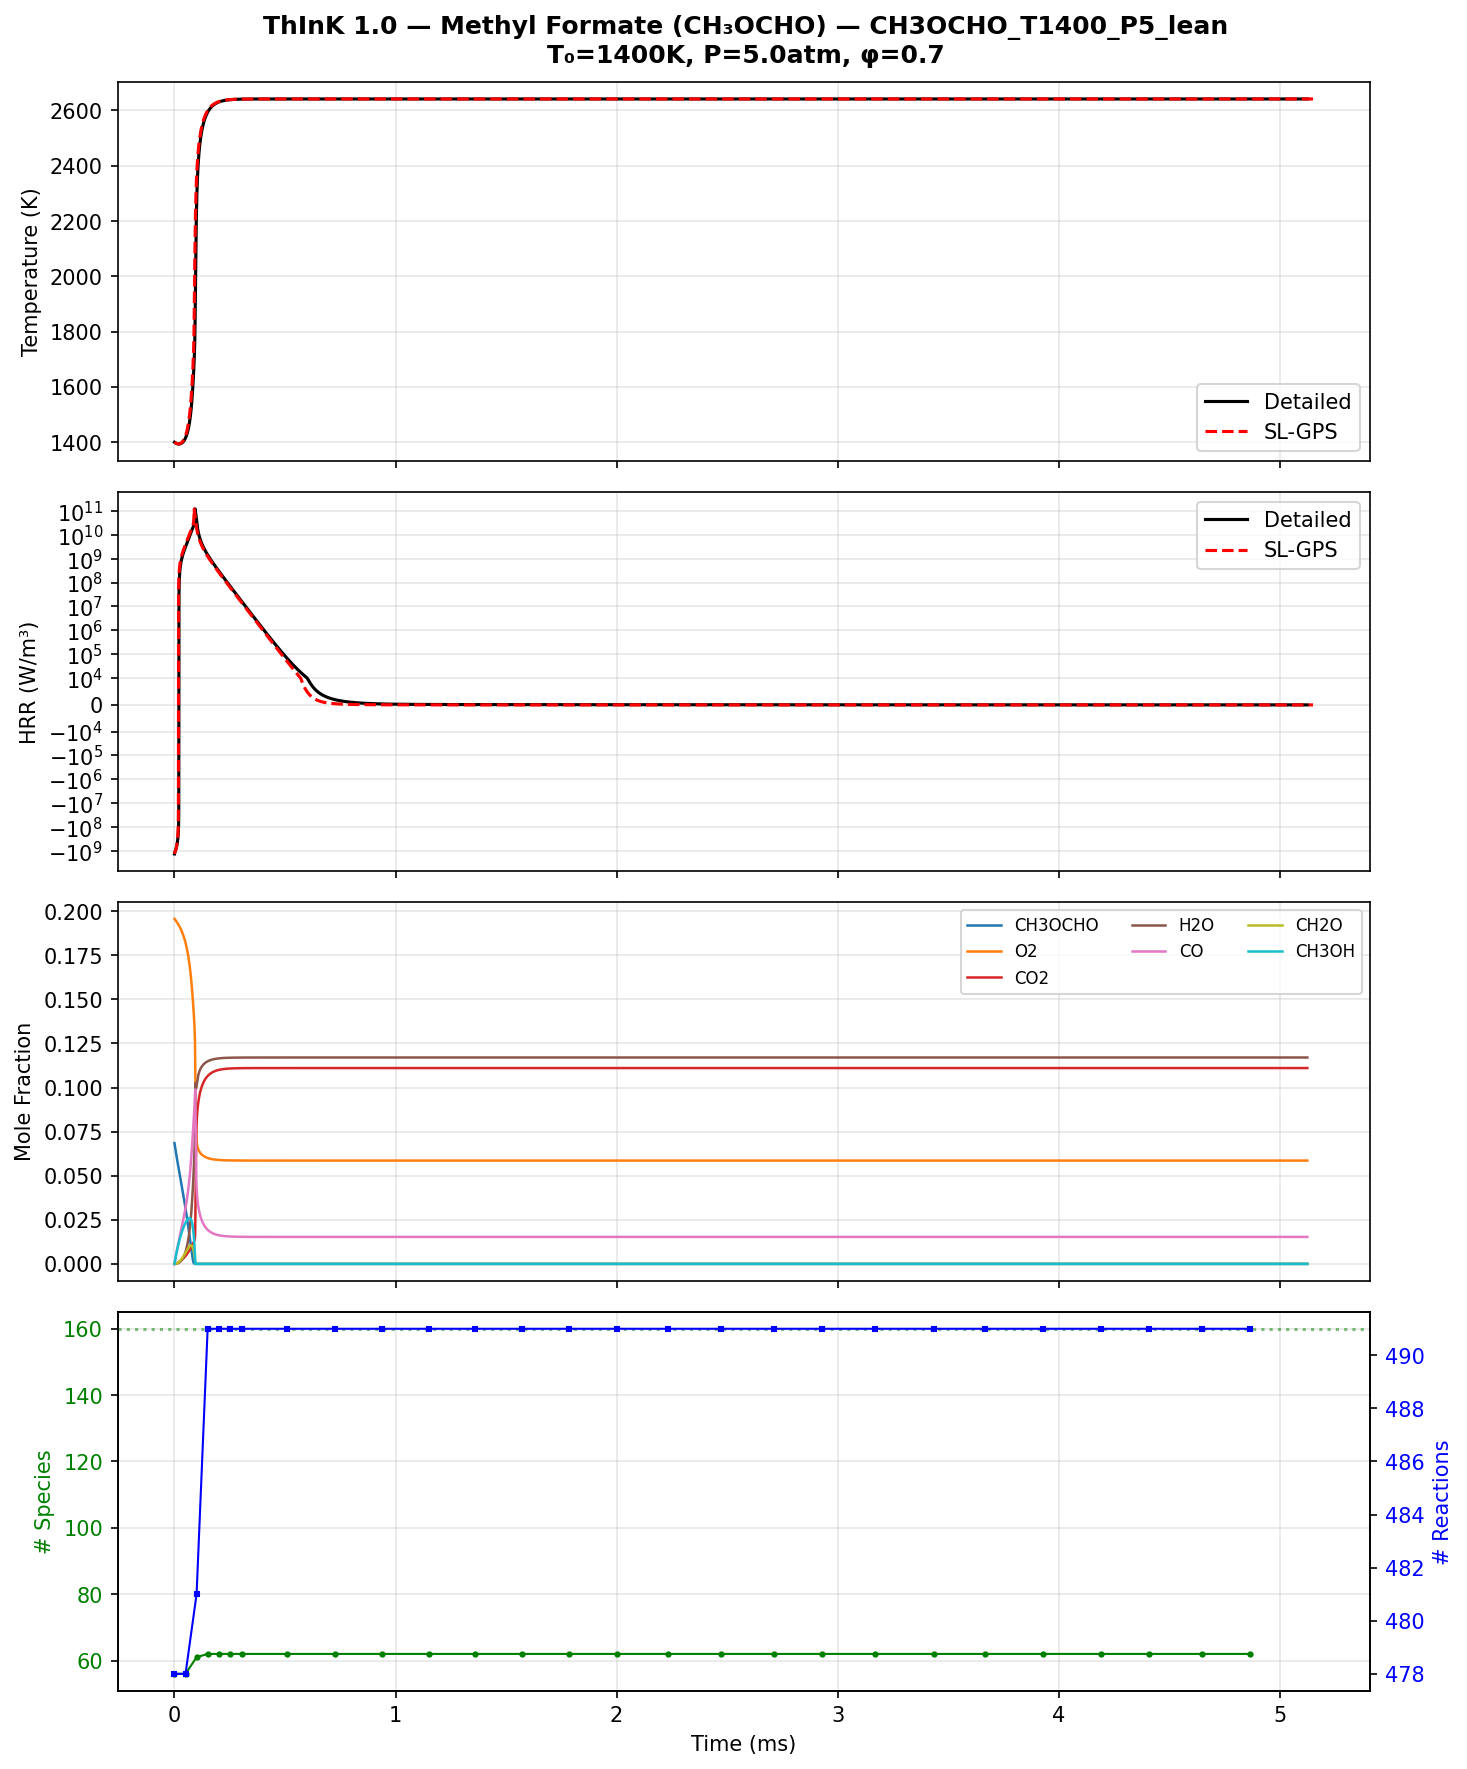
\includegraphics[width=0.95\textwidth]{results/ch3ocho/CH3OCHO_T1400_P5_lean.png}
    \caption{CH$_3$OCHO Case 8: $T_0=1400$~K, $P=5$~atm, $\phi=0.7$. Fuel-lean. Ignition delay error: 4.5\%.}
    \label{fig:ch3ocho_case8}
\end{figure}

\subsection{Summary}

\begin{figure}[H]
    \centering
    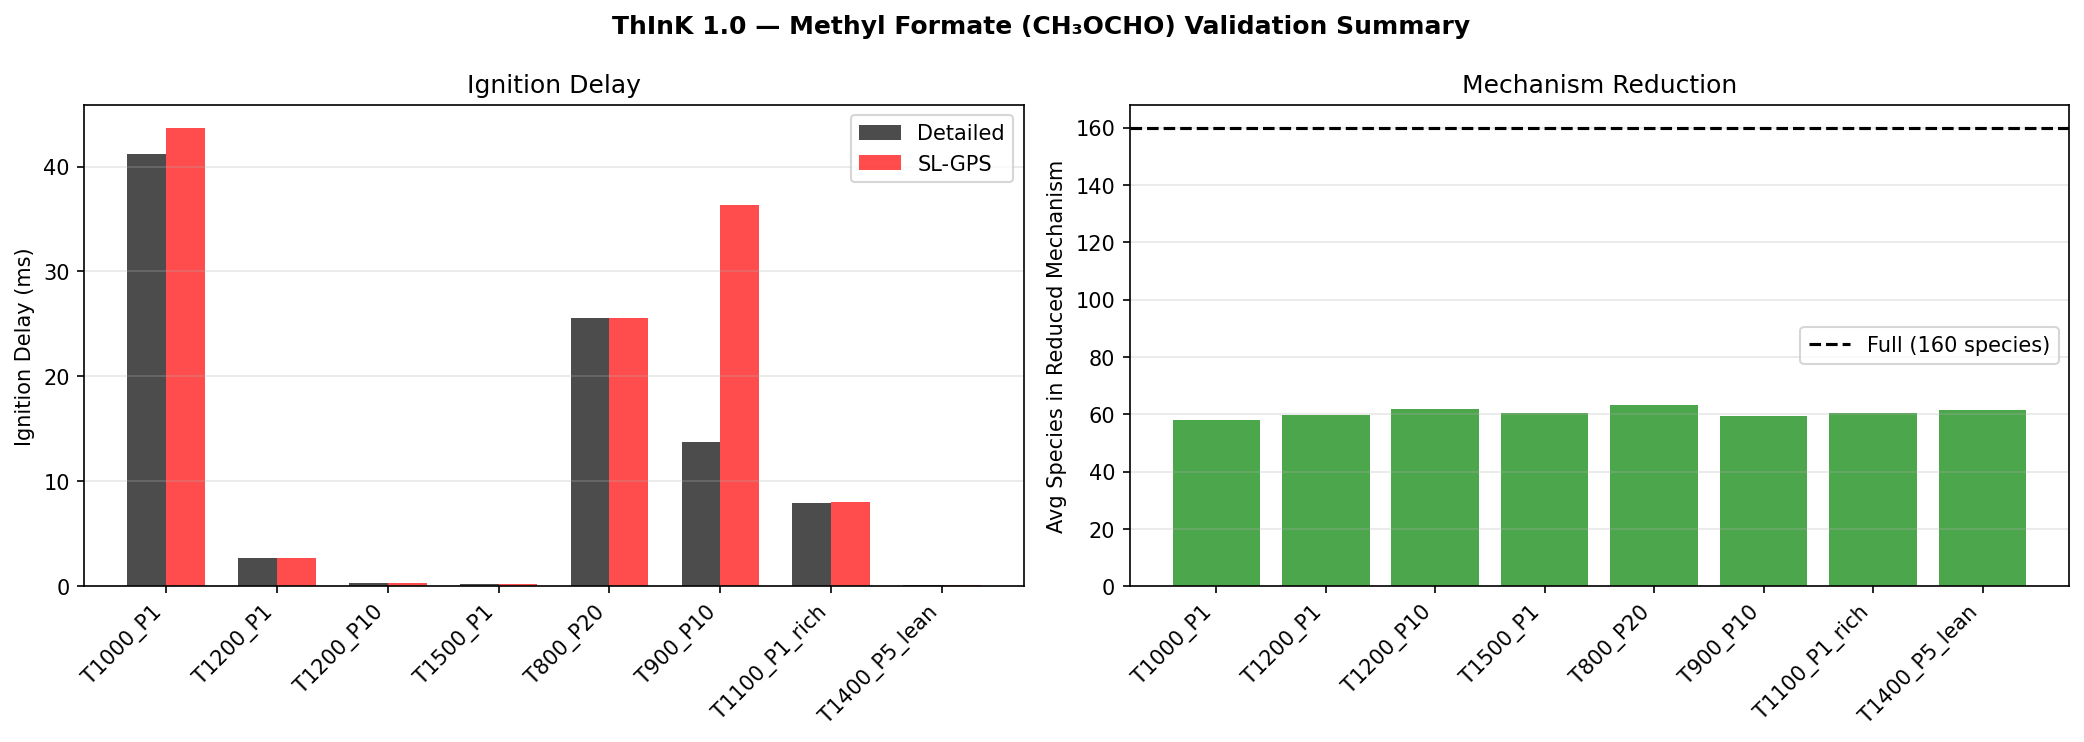
\includegraphics[width=0.95\textwidth]{results/ch3ocho/CH3OCHO_summary.png}
    \caption{CH$_3$OCHO validation summary. Left: ignition delay comparison (detailed vs.\ SL-GPS). Right: average mechanism size.}
    \label{fig:ch3ocho_summary}
\end{figure}

\begin{table}[H]
\centering
\caption{CH$_3$OCHO validation results summary.}
\label{tab:ch3ocho_results}
\begin{tabular}{lccccccc}
\toprule
\textbf{Case} & \textbf{$T$ (K)} & \textbf{$P$ (atm)} & \textbf{$\phi$} & \textbf{$\tau_{\text{det}}$ (ms)} & \textbf{$\tau_{\text{SL}}$ (ms)} & \textbf{Error (\%)} & \textbf{Pass} \\
\midrule
T1000\_P1        & 1000 &  1 & 1.0 & 41.240 & 43.698 &   6.0 & \checkmark \\
T1200\_P1        & 1200 &  1 & 1.0 &  2.660 &  2.665 &   0.2 & \checkmark \\
T1200\_P10       & 1200 & 10 & 1.0 &  0.280 &  0.290 &   3.4 & \checkmark \\
T1500\_P1        & 1500 &  1 & 1.0 &  0.226 &  0.224 &   0.9 & \checkmark \\
T800\_P20        &  800 & 20 & 1.0 & 25.529 & 25.597 &   0.3 & \checkmark \\
T900\_P10        &  900 & 10 & 1.0 & 13.716 & 36.373 & 165.2 & $\times$ \\
T1100\_P1\_rich  & 1100 &  1 & 1.3 &  7.968 &  8.071 &   1.3 & \checkmark \\
T1400\_P5\_lean  & 1400 &  5 & 0.7 &  0.094 &  0.090 &   4.5 & \checkmark \\
\midrule
\multicolumn{4}{l}{\textbf{Overall}} & \multicolumn{2}{c}{\textbf{7/8 passed}} & \textbf{22.7} & \\
\multicolumn{4}{l}{\textbf{Excl.\ outlier (T900\_P10)}} & \multicolumn{2}{c}{\textbf{7/7 passed}} & \textbf{2.4} & \\
\bottomrule
\end{tabular}
\end{table}

\begin{table}[H]
\centering
\caption{CH$_3$OCHO mechanism reduction summary.}
\label{tab:ch3ocho_reduction}
\begin{tabular}{lcc}
\toprule
\textbf{Metric} & \textbf{Value} \\
\midrule
Detailed mechanism species & 160 \\
Mean reduced species & 61 \\
Mean reduction & 62\% \\
Always species (unconditional) & 14 \\
Variable species (ANN-predicted) & 63 \\
Never species (excluded) & 83 \\
\bottomrule
\end{tabular}
\end{table}

% =============================================================================
\section{Discussion}
\label{sec:discussion}
% =============================================================================

\subsection{Accuracy}

Across 7 of 8 validation cases, SL-GPS reproduces ignition delay times with a mean error of 2.4\%, demonstrating that the ANN accurately captures the GPS species selection for methyl formate combustion. Temperature profiles, heat release rates, and major species evolution closely match the detailed mechanism.

\subsection{Failed Case Analysis}

The T900\_P10 case ($T_0=900$~K, $P=10$~atm) exhibits a 165\% ignition delay error. This condition falls in the low-temperature / intermediate-pressure regime where:
\begin{itemize}
    \item Methyl formate undergoes complex low-temperature oxidation pathways
    \item The competition between thermal decomposition and H-abstraction channels is sensitive to radical pool composition
    \item The ANN may lack sufficient training data at this specific condition
\end{itemize}
Potential remedies include:
\begin{enumerate}
    \item Increasing \texttt{n\_cases} from 15 to 30+ to improve low-$T$ coverage
    \item Adding targeted training conditions at 850--950~K, 5--15~atm
    \item Widening the neural network architecture (e.g., $2 \times 64$ neurons)
\end{enumerate}

\subsection{Mechanism Reduction}

The adaptive SL-GPS approach reduces the ThInK~1.0 mechanism from 160 species to an average of 61 active species (62\% reduction). The species count varies dynamically:
\begin{itemize}
    \item \textbf{Pre-ignition:} $\sim$55--60 species active
    \item \textbf{During ignition:} peak at $\sim$65 species as radical pool builds
    \item \textbf{Post-ignition:} relaxation to $\sim$58 species
\end{itemize}

% =============================================================================
\section{Reproducibility}
\label{sec:reproducibility}
% =============================================================================

All scripts are in \texttt{validation/ThinkMechanism/}:

\begin{lstlisting}[language=bash]
# Full pipeline (data gen + training + validation + plots)
cd validation/ThinkMechanism
python run_pipeline_ch3ocho.py   # ~47 min total
\end{lstlisting}

\subsection{Prerequisites}

\begin{itemize}
    \item Cantera $\geq$ 3.0.0 with ThInK 1.0 mechanism (\texttt{ThInK\_1.0\_Mech.yaml})
    \item Python 3.10+, TensorFlow 2.x, NumPy, scikit-learn, Matplotlib, Joblib
    \item $\geq$8 CPU cores recommended (parallel data generation and ensemble training)
\end{itemize}

\subsection{Output Files}

\begin{table}[H]
\centering
\caption{Pipeline output files.}
\label{tab:outputs}
\begin{tabular}{ll}
\toprule
\textbf{Path} & \textbf{Description} \\
\midrule
\texttt{models/ch3ocho/model.h5} & Best trained ANN model \\
\texttt{models/ch3ocho/scaler.pkl} & MinMaxScaler for input normalization \\
\texttt{data/train\_ch3ocho/data.csv} & Training state vectors \\
\texttt{data/train\_ch3ocho/species.csv} & GPS species importance labels \\
\texttt{results/ch3ocho/*.png} & Per-case validation plots \\
\texttt{results/ch3ocho/*.pkl} & Raw simulation data \\
\texttt{results/ch3ocho/CH3OCHO\_summary.png} & Summary comparison plot \\
\texttt{results/ch3ocho/validation\_report.txt} & Text report \\
\bottomrule
\end{tabular}
\end{table}

% =============================================================================
\begin{thebibliography}{9}

\bibitem{think1}
ThInK~1.0: A comprehensive thermochemical and kinetic model for oxygenated C$_1$--C$_3$ fuels,
\emph{Combustion and Flame}, 2025.

\bibitem{slgps}
R.~Mishra, A.~Nelson, D.~Jarrahbashi,
``Adaptive global pathway selection using artificial neural networks: A-priori study,''
\emph{Combustion and Flame}, vol.~244, p.~112279, 2022.

\bibitem{gps}
X.~Gao, S.~Yang, W.~Sun,
``A global pathway selection algorithm for the reduction of detailed chemical kinetic mechanisms,''
\emph{Combustion and Flame}, vol.~167, pp.~238--247, 2016.

\end{thebibliography}

\end{document}
